Dado que en este proyecto se ha planteado la construcción de un manipulador o brazo robótico, los únicos actuadores empleados han sido motores, los cuales dotan de movilidad a la estructura física del brazo.

Cabe destacar que, debido a la forma de la estructura física del brazo y dado a que el mismo tiene tres articulaciones móviles, se han empleado tres motores principales en cada una de ellas y un motor auxiliar en el extremo del manipulador.

Existen varios tipos de motores eléctricos que pueden ser usados para dotar de movilidad a proyectos de robótica de pequeña escala. Sin embargo los principales tipos se pueden aglutinar en las siguientes tres categorías:

\begin{itemize}
    \item Motores de corriente continua: son los motores eléctricos más sencillos y básicos. Debido a esto, realizar el control de la posición angular del eje y su velocidad de rotación es complicado y requiere aplicar técnicas de control de lazo cerrado. Además, el control físico de este tipo de motores se lleva a cabo mediante una señal \ac{PWM} actuando sobre un puente H.
 
    \begin{figure}[htbp]
    \centering
    \subfigure[Motor DC real \cite{7759009FCCCDatasheetHoja}]{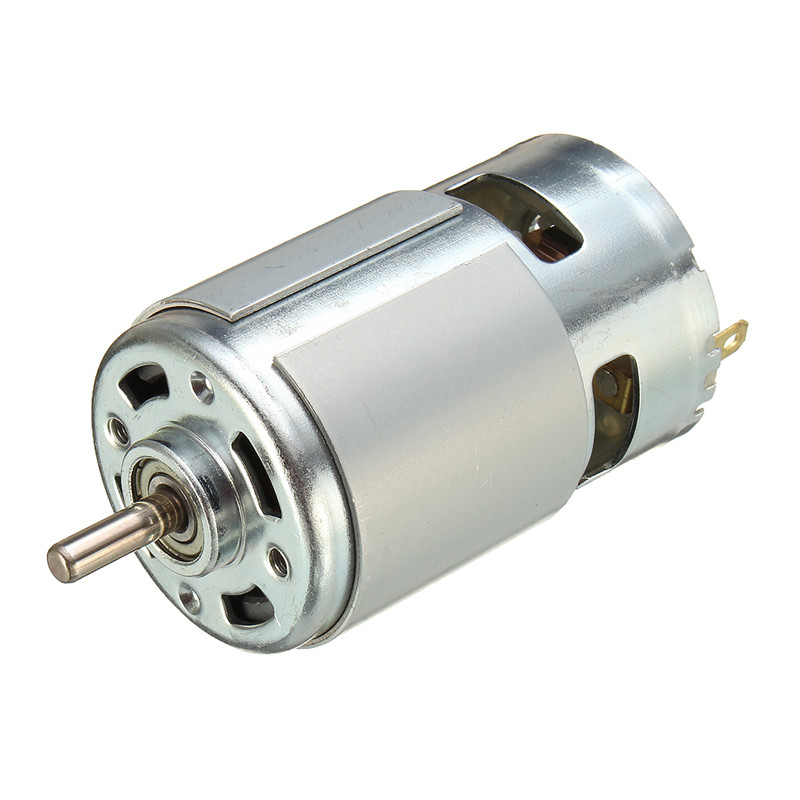
\includegraphics[width=40mm]{pictures/DcMotor.jpeg}}
    \subfigure[Funcionamiento \cite{MotorCorrienteContinua2020}]{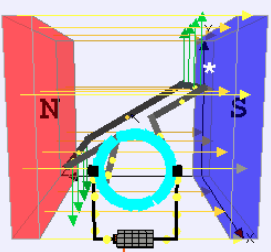
\includegraphics[width=40mm]{pictures/Motor DC Magnetic.png}}
    \caption{Motor de corriente continua} \label{fig:lego}
    \end{figure}


    \item Motores paso a paso: se trata de motores eléctricos más complejos que ofrecen una precisión muy alta en cuanto a  control de posición y velocidad, ya que descomponen su movimiento en pasos de longitud constante. En este tipo de motores se puede realizar control de velocidad y posición del eje del motor mediante técnicas de control de lazo abierto, dado que en este tipo de motores se controla el número de pasos que da el motor, así como cada cuanto tiempo se produce un paso. Este tipo de motores suelen necesitar un \textit{driver} específico para ser controlados.
    
    \begin{figure}[H]
    \centering
    \subfigure[Motor real \cite{banggood.com3pcs42mm12V}]{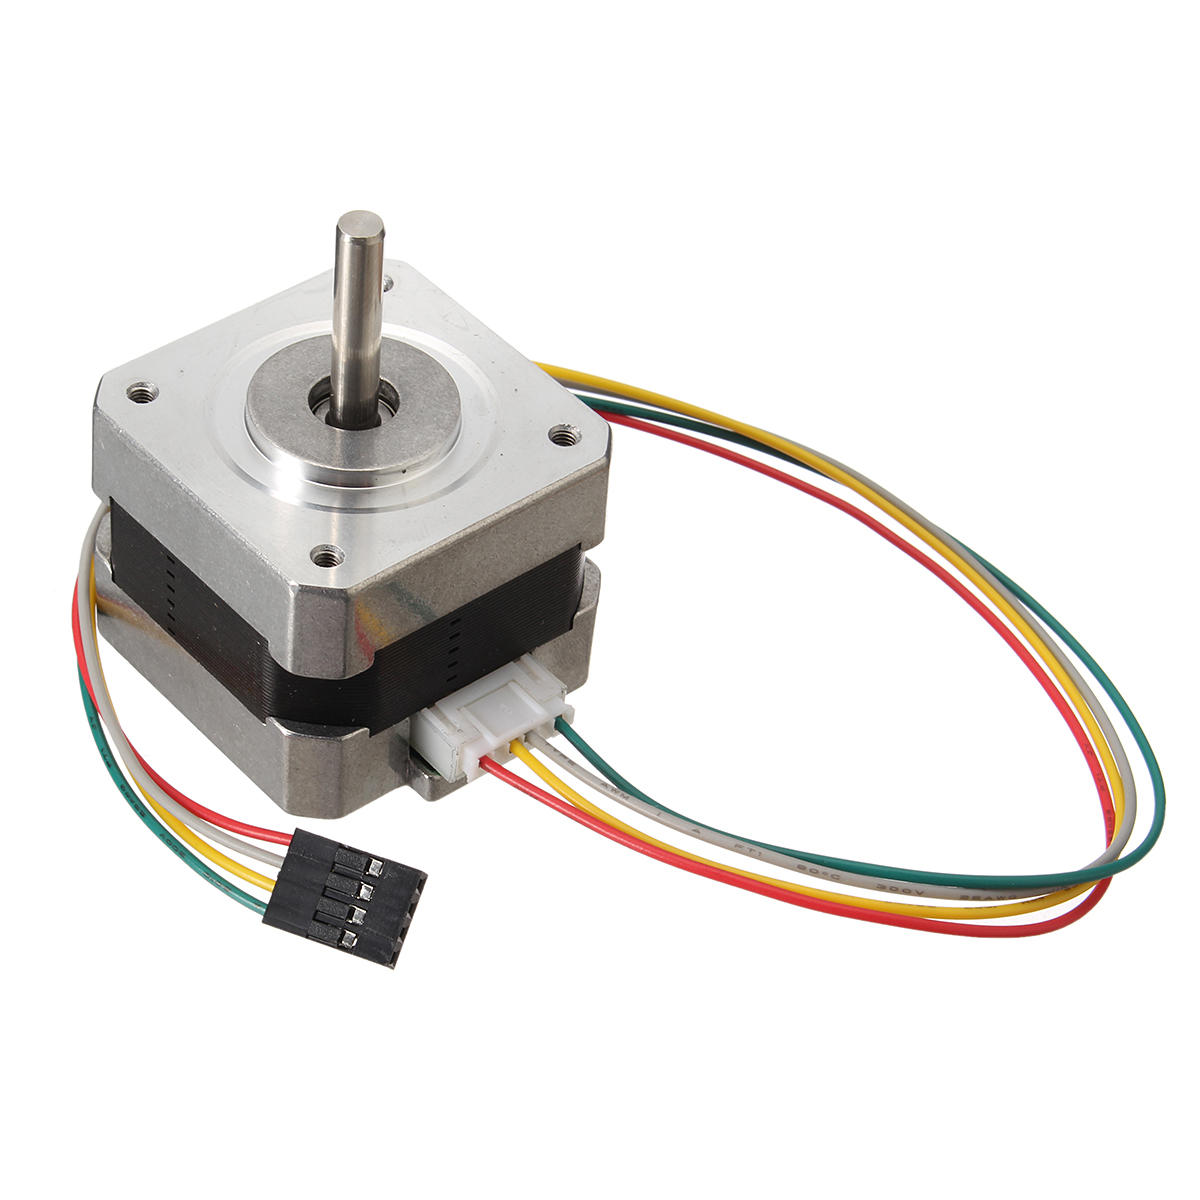
\includegraphics[width=56mm]{pictures/PasoPasoMotor.jpg}}
    \subfigure[Funcionamiento \cite{StepperMotorsTypes}]{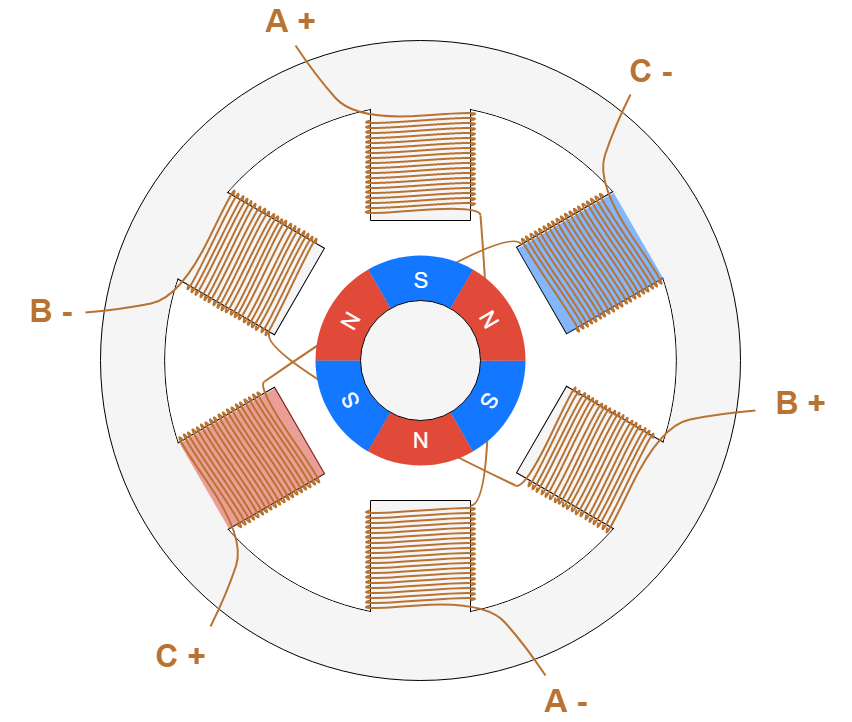
\includegraphics[width=56mm]{pictures/MotorPasoPasoMagnetic.png}}
    \caption{Motor paso a paso} \label{fig:lego}
    \end{figure}
  
    \item Servomotores: se trata de motores de corriente continua que incorporan un sistema de control de posición de lazo cerrado. Por ello, este tipo de motores ofrecen un control muy simple de la posición angular del eje del motor. A través de una señal \ac{PWM} enviada al motor, se puede establecer una posición consigna que el eje del motor debe cumplir. Estos motores incluyen un sensor de posición (encoder, potenciómetro solidario al eje o similar) que determina la posición angular del eje del motor y una unidad de control que verifica la posición actual del eje en comparación con la posición de consigna establecida, realizando las correcciones necesarias hasta alcanzar dicha posición angular.
    %%Poner foto
    
    \begin{figure}[H]
    \centering
    \subfigure[Servomotor real \cite{MiniServomotorEbotics}]{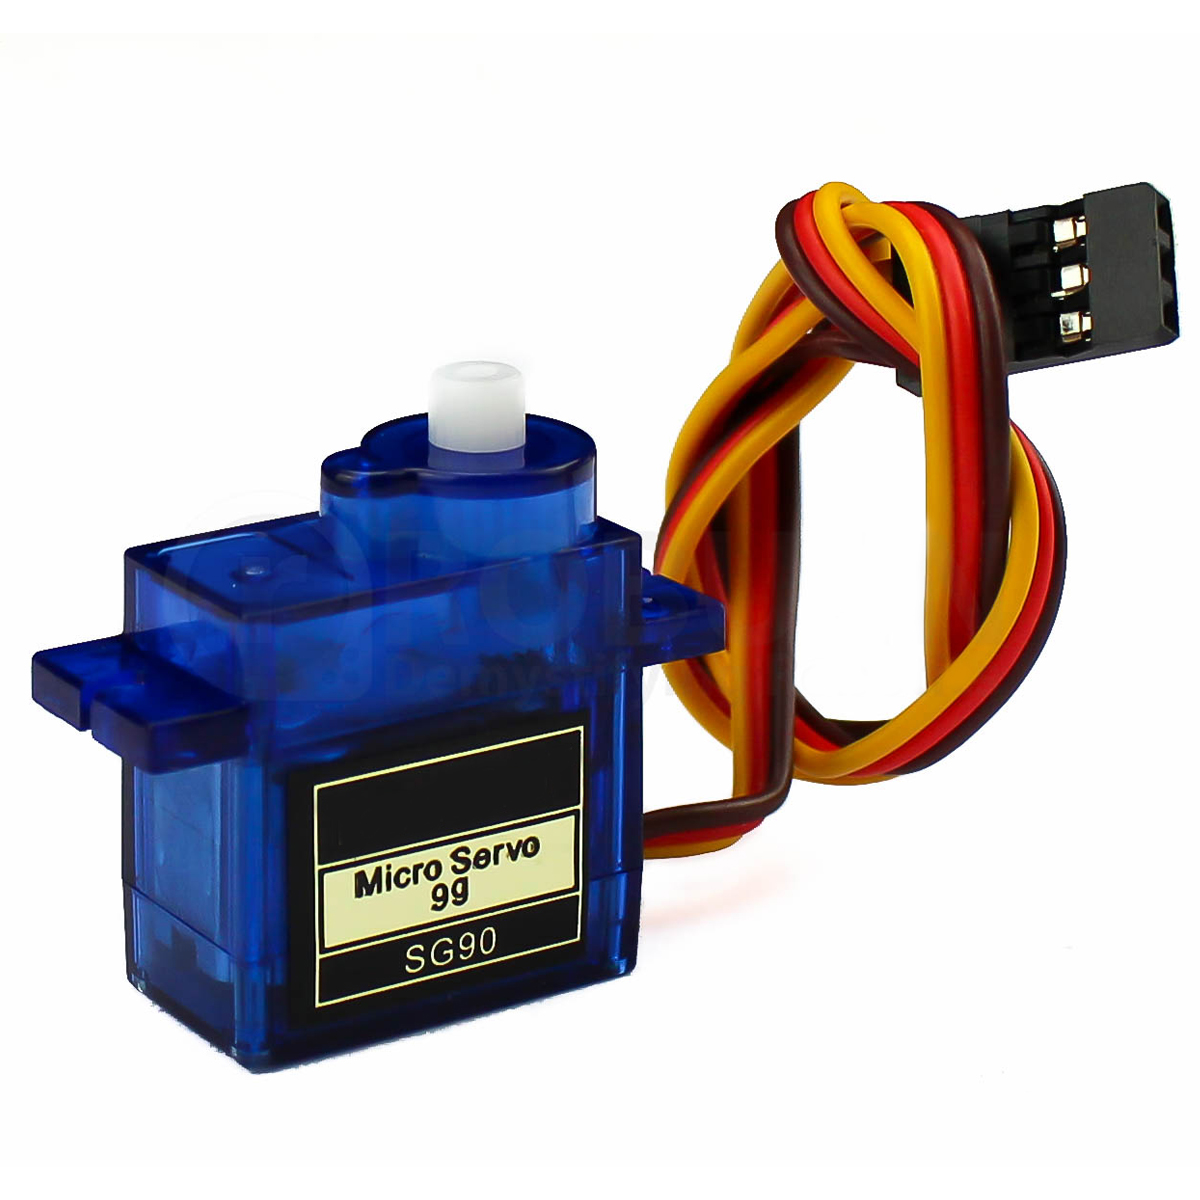
\includegraphics[width=50mm]{pictures/Servo.jpg}}
    \subfigure[Funcionamiento \cite{HowServoMotor2019}]{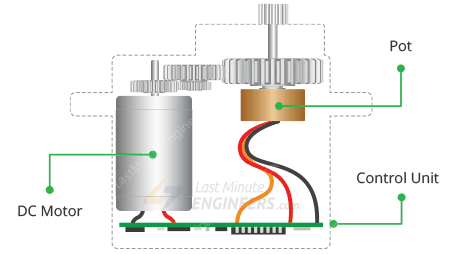
\includegraphics[width=80mm]{pictures/Servo-Motor-Internal-Structure-Illustration.png}}
    \caption{Servomotor de corriente continua} \label{fig:lego}
    \end{figure}
    
\end{itemize}

Tras analizar los diferentes tipos de motores anteriormente expuestos, se ha decidido utilizar servomotores para dotar de movilidad al brazo robótico. Esta decisión se fundamenta en los siguientes motivos:
\begin{itemize}

    \item A diferencia de los motores paso a paso o motores de corriente continua, no se suele necesita ningún tipo de circuito externo, driver o puente H para controlar un servomotor; únicamente se debe alimentar el motor y proporcionar una señal de control.
    
    \item Este tipo de motores ofrece un control de posición preciso y simple mediante una señal \ac{PWM}. A pesar de que dicho control de posición se realiza mediante lazo cerrado internamente dentro del motor, desde un punto de vista externo, no se necesita ningún tipo de realimentación externa.
    
    \begin{figure}[h!]
    \centering 
    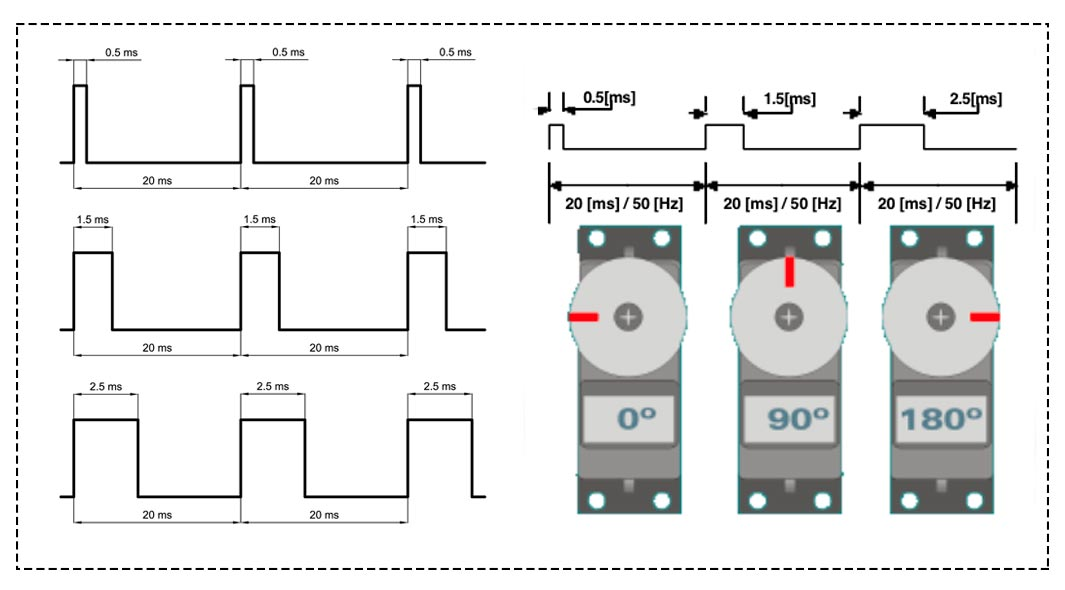
\includegraphics[width=.6\linewidth]{pictures/Senal_PWM.jpg}
    \caption{Ejemplo genérico de control de posición mediante señal PWM \cite{ZonaMakerServomotores}.}
    \label{fig:}
    \end{figure}
    
    \item Se trata de motores que se adaptan muy bien para proyectos de robótica de pequeña escala, debido a su bajo coste y sencillez de uso.
    
    \item Este tipo de motores está muy extendido en el mercado y existen numerosos modelos con diferentes potencias, tamaños, etc.
\end{itemize}

Es importante destacar que existen dos tipos de servomotores:
\begin{itemize}
    \item Servomotores de giro limitado: son aquellos servomotores que tienen un rango de rotación limitado, el cual suele ser normalmente de 180º. Son el tipo de servomotor más sencillo.
    \item Servomotores de giro continuo: son aquellos servomotores que tienen rango completo de giro, es decir, pueden realizar giros sin limitación de recorrido.
\end{itemize}

Dado que ninguna de las articulaciones del motores está diseñada para realizar giros de más de 180º, se han empleado servomotores de giro limitado.

Otro de los datos que es importante clarificar antes de tomar la decisión de que motores van a ser usados en un proyecto de robótica, es la carga máxima que va a tener que desplazar el manipulador robótico. Este dato afecta principalmente al diseño de la estructura física del brazo y a la potencia de los motores escogidos, en especial, el torque que ejercen. 

Finalmente, el modelo de servomotor elegido para las articulaciones ha sido el \textit{Parallax 900-00005 Standard Servo} el cual tiene las siguientes características técnicas:

\begin{itemize}
    \item Servomotor de rango limitado de 180º.
    \item Control mediante señal \ac{PWM} de 50Hz.
    \item Alimentación de entre $4V$ y $6V$, utilizando entre $15mA$ y $200mA$. Potencia nominal de $140mA$.
    \item Torque máximo ejercido de $27N\cdot cm$, es decir aproximadamente $2.75 Kgf\cdot cm$. 
    \item Conociendo el torque ejercido por los servomotores y área de trabajo del manipulador, mostrada en la figura \ref{fig:pArm_working_area}, se pueden realiza algunos cálculos para deducir cual será la carga máxima que podrá soportar el brazo robótico:
    \begin{itemize}
        \item En la zona de trabajo en la cual el brazo robótico esta menos extendido, y por lo tanto situación  en la que el esfuerzo es mínimo sobre la estructura del manipulador, los motores aplican su fuerza a 8.1 cm del extremo del robot. Dado que el torque es generado es de aproximadamente $2.75 Kgf\cdot cm$, se podría levantar una masa de aproximadamente 300g.
        
        \item En la zona de trabajo en la cual el brazo robótico esta más extendido, y por lo tanto situación en la que el esfuerzo es máximo sobre la estructura del robot, los motores aplican su fuerza a 34.6 cm del extremo del robot. Dado que el torque es generado es de aproximadamente $2.75 Kgf\cdot cm$, se podría levantar una masa de aproximadamente 80g.
        
        \item Teniendo en cuenta los cálculos anteriores, se recomienda que la carga máxima del manipulador sea de entre 150g y 60g, siempre teniendo en cuenta las zonas de trabajo en las que se vaya a desplazar la carga para tener garantías de que el desplazamiento es seguro.
    \end{itemize}
    \item Peso de 44g.
    \item Dimensiones 406 x 55,8 x 19 mm
\end{itemize}

\begin{figure}[H]
    \centering 
    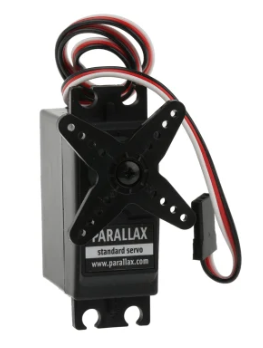
\includegraphics[width=.35\linewidth]{pictures/ServoParallax.PNG}
    \caption{Servomotor Parallax utilizado \cite{90000005ServomotorParallax}}
    \label{fig:}
\end{figure}

Teniendo en cuenta los datos técnicos anteriores, este modelo de servomotor se adapta perfectamente a las características del brazo robótico que se ha desarrollado, cumpliendo todas la cualidades deseadas para que el funcionamiento del brazo robótico sea correcto.